\documentclass[11pt]{article}
\usepackage[T1]{fontenc}
\usepackage{lmodern,microtype}
\usepackage[margin=1in]{geometry}
\usepackage{amsmath,amssymb,amsthm,mathtools,enumitem,booktabs}
\usepackage{graphicx,tikz}
\usepackage{float}
\floatstyle{plain}
\newfloat{algorithm}{tbp}{loa}
\floatname{algorithm}{Algorithm}
\usepackage{pgfplots}
\pgfplotsset{compat=1.18}
\usetikzlibrary{arrows.meta,positioning,shapes.geometric}
\definecolor{cellblue}{RGB}{40,95,150}
\definecolor{cellorange}{RGB}{190,100,25}
\usepackage[hidelinks]{hyperref}
\setlength{\emergencystretch}{3em}
\newtheorem{theorem}{Theorem}[section]
\newtheorem{lemma}[theorem]{Lemma}
\newtheorem{proposition}[theorem]{Proposition}
\newtheorem{corollary}[theorem]{Corollary}
\theoremstyle{definition}\newtheorem{definition}{Definition}[section]
\theoremstyle{remark}\newtheorem{remark}[theorem]{Remark}
\newcommand{\R}{\mathbb R}\newcommand{\Q}{\mathbb Q}\newcommand{\Z}{\mathbb Z}
\newcommand{\eps}{\varepsilon}
\newcommand{\poly}{\operatorname{poly}}
\newcommand{\osc}{\operatorname{osc}}
\newcommand{\bits}{\operatorname{bits}}
\newcommand{\norm}[1]{\lVert#1\rVert}
\title{A Short Proof of a Range-Relative FPTAS\\for Polynomial Integer Optimization over Bounded Polyhedra}
\author{Robert Hildebrand\thanks{Developed with assistance from OpenAI's Codex assistant; see the detailed AI-assistance and contribution disclosure at the end of the paper.}}
\date{October 14, 2026}
\begin{document}
\maketitle
\begin{abstract}
We give a short proof of a fully polynomial-time range-relative approximation scheme for polynomial optimization over the integer points of a bounded rational polyhedron in fixed dimension. Boundedness supplies a finite slack decomposition and a finite integer objective range. The proof combines the reflecting-set decomposition of Cook, Hartmann, Kannan, and McDiarmid with Markov's inequality and uses one integer linear feasibility query per refined cell. The running time is polynomial in the input encoding length, the numerical degree, and the reciprocal accuracy.
\end{abstract}

\section{Introduction and main result}

Let $P=\{\mathbf{x}\in\R^d:A\mathbf{x}\le\mathbf b\}$ be a bounded rational polyhedron, with $A\in\Q^{m\times d}$ and $\mathbf b\in\Q^m$, and let $f\in\Z[x_1,\ldots,x_d]$. We study
\begin{equation}\label{eq:problem}
 \begin{aligned}
 \min\quad & f(\mathbf{x})\\
 \text{s.t.}\quad & A\mathbf{x}\le\mathbf b,\\
 & \mathbf{x}\in\Z^d.
 \end{aligned}
\end{equation}
When $P\cap\Z^d\ne\varnothing$, choose minimizers and maximizers $\mathbf{x}_{\min},\mathbf{x}_{\max}$ and write $f_{\min}=f(\mathbf{x}_{\min})$ and $f_{\max}=f(\mathbf{x}_{\max})$.

We use $d$ for dimension, $D$ for total degree, and $\mathbf{x}_{\eps}$ for the returned point, following~\cite{DHKW08}. The range-relative guarantee is their weak approximation guarantee, stated here for minimization. It is invariant under translation of the objective. It is different from a multiplicative approximation to a nonnegative minimum.

De Loera, Hemmecke, K\"oppe, and Weismantel established fully polynomial approximation schemes based on short rational generating functions, including nonnegative polynomial maximization and range-relative approximation of arbitrary polynomial objectives in fixed dimension \cite{DHKW06,DHKW08}. Del Pia gives a geometric range-relative approximation algorithm for bounded mixed-integer quadratic programs with fixed quadratic rank and fixed number of integer variables \cite{DelPia}. We give an alternative construction for the bounded, pure-integer problem. The purpose is to obtain a short proof using linear feasibility, with explicit dependence on the encoding length.

\emph{The common geometric ingredient is a decomposition by relative slack scales.} The dyadic reflecting sets of Cook--Hartmann--Kannan--McDiarmid (CHKM) are central to their integer-hull analysis~\cite{CHKM}. Symmetric displacement covers likewise underpin the quadratic and cubic algorithms of Ari and Hildebrand~\cite{AHIQP,AH}. In parallel work on exact integer quadratic programming, Wei explicitly uses dyadic grouping of constraint slacks to obtain regions supporting two-sided feasible moves~\cite[Section~1.1]{Wei}. These uses suggest that relative-slack decompositions are a useful common tool for polynomial integer optimization: they convert proximity measured against the constraints into feasible algebraic comparisons, without reference to objective coefficients.

Here refinement strengthens one-step reflection to a long feasible arithmetic progression. Restricting a degree-$D$ polynomial to that progression and applying Markov's inequality then yields an objective-independent representative set that approximates both integer extrema; see Proposition~\ref{prop:extrema}. Thus the geometric cover serves all polynomial objectives of the prescribed degree simultaneously. The essential feature is multiplicative control of positive slacks, not the choice of base two: Remark~\ref{rem:slack-characterization} makes the connection to extrapolation exact. Related continuous sampling arguments based on Markov inequalities and norming meshes appear in Piazzon and Vianello~\cite{PV}; here the samples remain feasible integer points, so the error is measured against the integer objective range.

\begin{center}
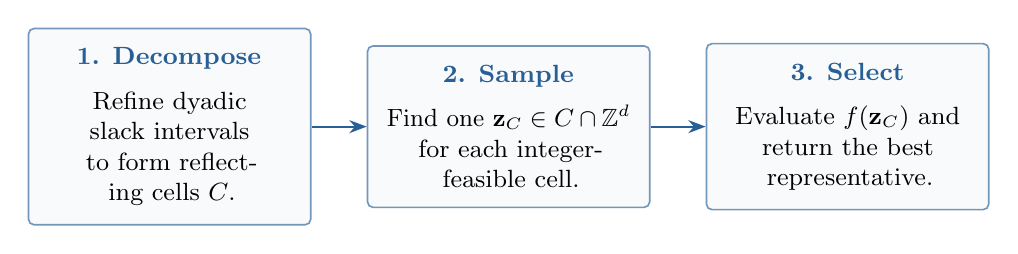
\begin{tikzpicture}[
  stage/.style={draw=cellblue!65,line width=.6pt,rounded corners=2pt,
    fill=cellblue!3,text width=.255\textwidth,minimum height=2.05cm,
    inner sep=7pt,align=center,font=\small},
  flow/.style={-{Stealth[length=2.2mm]},line width=.8pt,cellblue},
  node distance=7mm]
\node[stage] (decompose) {
  {\color{cellblue}\bfseries 1. Decompose}\\[5pt]
  Refine dyadic slack intervals\\
  to form reflecting cells $C$.
};
\node[stage,right=of decompose] (sample) {
  {\color{cellblue}\bfseries 2. Sample}\\[5pt]
  Find one $\mathbf z_C\in C\cap\Z^d$\\
  for each integer-feasible cell.
};
\node[stage,right=of sample] (select) {
  {\color{cellblue}\bfseries 3. Select}\\[5pt]
  Evaluate $f(\mathbf z_C)$ and\\
  return the best representative.
};
\draw[flow] (decompose)--(sample);
\draw[flow] (sample)--(select);
\end{tikzpicture}
\end{center}

No local approximation to the objective is optimized. Instead, reflection controls the error at a global optimum, which is enough to justify the final selection. Section~\ref{sec:cover} proves this estimate, Section~\ref{sec:algorithm} gives the algorithm and its bit complexity, and Section~\ref{sec:conclusion} discusses extensions and related decomposition methods.

More broadly, the method follows a decompose--solve--select pattern: a local error bound on the cell containing an optimum transfers to the best returned candidate. For polynomial optimization, this permits other cell decompositions or tractable local models when suitable error estimates are available.

The decomposition also connects to the geometric subdivision of Papadimitriou and Yannakakis~\cite{PY} and its use for affine slicing in Hildebrand, Weismantel, and Zemmer~\cite[Section~2]{HWZ}. Applying multiplicative bins to the slacks $s_i(\mathbf{x})=b_i-\mathbf a_i^\top\mathbf{x}$ gives the same relative-width property as our refined dyadic intervals: a bin $[a,(1+\delta)a]$ has width at most $\delta a$. Points in a common block therefore extend to feasible progressions of length $1/\delta$, with zero slacks handled separately. As in the proof of~\cite[Theorem~2.1]{HWZ}, the bins are pulled back to an arrangement in the original variable space $\R^d$; enumerating all combinations in the $m$-dimensional slack space would lose the fixed-dimensional complexity bound. Unlike the sliceable-objective framework of~\cite{HWZ}, our approximation argument uses Markov's inequality and measures error relative to the objective range.

To state the complexity bound precisely, we fix the following encoding convention. Vectors are columns and are written in bold. For an integer $u$, set $\langle u\rangle=1+\lceil\log_2(1+|u|)\rceil$. A rational number $u/v$ is stored in lowest terms with $v>0$, with size $\langle u/v\rangle=\langle u\rangle+\langle v\rangle$. For matrices, vectors, and lists, $\langle\cdot\rangle$ is the sum of the entry sizes together with the binary sizes of the dimensions and list lengths. The polynomial is supplied explicitly as
\[
 f(\mathbf{x})=\sum_{\alpha\in\mathcal A}c_\alpha\mathbf{x}^\alpha,
 \qquad c_\alpha\in\Z,\quad \alpha\in\Z_+^d,\quad |\alpha|_1\le D.
\]
Following~\cite{DHKW08}, coefficients are encoded in binary and exponent vectors in unary: each exponent $\alpha_j$ occupies $\alpha_j+1$ symbols. Thus $\langle f\rangle$ includes the coefficient sizes and $\sum_{\alpha\in\mathcal A}\sum_{j=1}^d(\alpha_j+1)$, together with dimensions and list lengths. Write $\varphi=\langle A,\mathbf b,f,\eps\rangle$ for the total input encoding size. We compute $D=\max\{1,\deg f\}$ from the nonzero monomials, taking $D=1$ for the zero polynomial; no separate degree input is needed. We retain $D$ explicitly in the running-time bound to show its contribution.

\begin{definition}[Range-relative FPTAS]\label{def:fptas}
Under the encoding convention above and for fixed dimension $d$, a range-relative fully polynomial-time approximation scheme is an algorithm that, for every rational $0<\eps\le1$, reports infeasibility when $P\cap\Z^d=\varnothing$, and otherwise returns $\mathbf{x}_{\eps}\in P\cap\Z^d$ satisfying
\begin{equation}\label{eq:guarantee}
 0\le f(\mathbf{x}_{\eps})-f_{\min}\le\eps(f_{\max}-f_{\min}).
\end{equation}
Its running time is polynomial in the total input encoding size $\varphi$ and $1/\eps$. The polynomial may depend on the fixed dimension. This is the fully polynomial-time weak-approximation notion of~\cite{DHKW08}. The maximization definition uses $f_{\max}-f(\mathbf{x}_{\eps})$ on the left.
\end{definition}

All complexity statements below count bit operations. The function $\poly$ denotes a polynomial with an absolute exponent, independent of $d,D,\eps$; different occurrences may denote different polynomials. Logs are base two unless indicated otherwise.

\begin{theorem}[Polynomial approximation by reflecting cells]\label{thm:main}
Let $d\ge1$ and let $P=\{\mathbf{x}\in\R^d:A\mathbf{x}\le\mathbf b\}$ be bounded, with $A\in\Z^{m\times d}$ and $\mathbf b\in\Z^m$, let $f\in\Z[x_1,\ldots,x_d]$, and put $D=\max\{1,\deg f\}$, with $D=1$ when $f=0$. For rational $0<\eps\le1$, let $\varphi=\langle A,\mathbf b,f,\eps\rangle$ be the total input encoding size.
There is a deterministic algorithm that reports infeasibility or returns $\mathbf{x}_{\eps}\in P\cap\Z^d$ satisfying~\eqref{eq:guarantee}, in at most
\begin{equation}\label{eq:runtime-coarse}
 \left(\frac{\varphi D}{\eps}\right)^{O(d)}
\end{equation}
bit operations, with an absolute constant in the $O(d)$ exponent.
\end{theorem}

Since the input explicitly lists the $m$ inequalities in $d$ variables, $m,d\le\varphi$; their separate factors in the detailed running-time bound are therefore absorbed into the base $\varphi$ and the $O(d)$ exponent in~\eqref{eq:runtime-coarse}. The dependence on dimension remains explicit in that exponent. More precisely, for fixed $P,D,d$, the algorithm makes $O(\eps^{-d/2})$ integer-feasibility queries; the detailed running-time bound in the proof retains the factor $D^2/\sqrt\eps$.

Rational inequalities can be normalized to integral data in polynomial time, as detailed below. Rational objective coefficients can likewise be reduced to integer coefficients by clearing denominators in polynomial time; positive scaling preserves the approximation guarantee, as in~\cite[Section~5]{DHKW08}. The remaining construction parameters and the exact feasibility-query count are introduced in the proof. For fixed $d$, the bound is polynomial in $\varphi$ and $1/\eps$, hence gives an FPTAS in Definition~\ref{def:fptas}. The same explicit bound remains valid for binary-encoded exponents, but then its numerical dependence on $D$ does not assert an FPTAS in the sparse binary input size.

\begin{corollary}[Nonnegative maximization]\label{cor:max}
Under the same assumptions and encoding conventions, if $f\ge0$ on $P\cap\Z^d$, choosing the largest objective value among the representatives yields
\[
 f(\mathbf{x}_{\eps})\ge(1-\eps)f_{\max}.
\]
Thus the construction gives a multiplicative FPTAS for nonnegative maximization under the encoding convention of Definition~\ref{def:fptas}.
\end{corollary}

\begin{corollary}[Mixed-integer approximation]\label{cor:mixed}
Fix the total dimension $d=d_c+d_i$. Let $P=\{\mathbf{x}\in\R^d:A\mathbf{x}\le\mathbf b\}$ be a bounded rational polyhedron and $f\in\Z[x_1,\ldots,x_d]$. Under the same encoding convention, for rational $0<\eps\le1$ there is an algorithm, polynomial in $\varphi=\langle A,\mathbf b,f,\eps\rangle$ and $1/\eps$, that reports infeasibility or returns
\[
 \mathbf{x}_{\eps}\in P\cap(\Q^{d_c}\times\Z^{d_i}),\qquad
 0\le f(\mathbf{x}_{\eps})-f_{\min}\le\eps(f_{\max}-f_{\min}),
\]
where the extrema are over $P\cap(\R^{d_c}\times\Z^{d_i})$. For nonnegative $f$ on this set, a multiplicative FPTAS for maximization is obtained as well.
\end{corollary}

Corollary~\ref{cor:mixed} combines our integer algorithm with the grid reduction of De Loera et al.~\cite{DHKW08}; it does not require a reflecting-cell cover of the entire mixed-integer feasible set.

\paragraph{Comparison with prior algorithms.}

The guarantee in~\eqref{eq:guarantee} is already provided by De Loera, Hemmecke, K\"oppe, and Weismantel~\cite{DHKW06,DHKW08}, whose generating-function algorithms run in time polynomial in the input length, numerical degree, and $1/\eps$ for fixed total dimension. Their integer nonnegative-maximization subroutine computes weighted lattice sums for $f^q$, with $q=O(1+\eps^{-1}\log N)$ and $N=|P\cap\Z^d|$; solution recovery uses further weighted sums on restricted polytopes~\cite[Section~3]{DHKW06}. Thus the work includes both Barvinok cone decomposition and subsequent symbolic calculations. A standard bound for the underlying lattice-point counting algorithm is $\langle A,\mathbf b\rangle^{O(d\log(d+1))}$~\cite[Theorem~2.3]{PakPanova}, whereas~\eqref{eq:runtime-coarse} gives $\varphi^{O(d)}$ for our entire algorithm when $D$ and $\eps$ are fixed. This compares available upper bounds, not a lower bound on their algorithm; the counting bound alone does not describe their full FPTAS. Their published analysis does not make all dimension-dependent exponents in the weighted-summation cost explicit. Our construction instead gives the explicit bound~\eqref{eq:runtime-coarse} through cell enumeration, integer linear feasibility, and exact polynomial evaluation, and produces a representative set independent of the objective coefficients. These differences do not establish practical superiority: our cell count can be large, while generating-function methods can benefit from small cone decompositions.

Del Pia's construction shares the partition-and-solve structure, but uses different geometry~\cite[Sections~3--6]{DelPia}. After transforming the problem to spherical form, the aligned-vector case partitions the $k$ quadratic coordinates into uniform boxes and minimizes an affine underestimator on each box by MILP; the remaining cases use flatness-based recursion. It does not use geometric slack bins. Our representatives instead require only feasibility because the reflected sample at an integer minimizer controls the first-order contribution.

For fixed quadratic rank $k$ and integer dimension $p$, Del Pia~\cite[Proposition~3 and Section~6.2]{DelPia} uses $O_{k,p}(1+\eps^{-k/2})$ mixed-integer linear optimization subproblems, with polynomial bit overhead for fixed $k,p$, while allowing variable continuous dimension. For our pure-integer algorithm, with fixed $P,D,d$, the counts proved in Section~\ref{sec:algorithm} are
\[
 O(\eps^{-d/2})\ \text{integer feasibility calls},\qquad
 O(\eps^{-(d+1)/2})\ \text{enumeration LP tests}.
\]
The per-test arithmetic has polynomial dependence on the encoding length $\langle\eps\rangle$. The feasibility-call exponent matches $k/2$ when $k=d$, but the enumeration overhead remains and the rank-sensitive bound for $k<d$ is not recovered. Our construction instead applies to arbitrary degree and supplies one objective-independent representative set. Its dimension-dependent factor includes both the constraint normals and right-hand sides through their binary encoding lengths; the displayed bound is not a fixed-parameter tractability claim in $d$.

\section{Reflecting cells and approximation}\label{sec:cover}

The proof separates the geometry of the feasible set from the behavior of the objective. We first partition the integer points into cells whose pairs extend to long feasible progressions. We then restrict the polynomial to such a progression through a global minimizer. The reflected point rules out a large first-order improvement in the backward direction, and a second-difference estimate controls the error of the forward representative. Neither the minimizer nor the objective range needs to be known by the algorithm.

The construction begins by making the slack gap explicit. If the input inequalities are rational, multiply each row by the product of the positive denominators in that row. This gives integral $A,\mathbf b$ in polynomial time, with total encoding length polynomial in the original input size $\varphi$. Each normalized entry has bit length $O(\varphi)$, since a row product has bit length at most the sum of its denominator bit lengths. The detailed bounds below refer to these normalized data; substituting their polynomial encoding bounds gives a bound in the original input length. No coefficient magnitude appears as a polynomial-time parameter.

Explicit equalities can be represented by pairs of inequalities. Lower-dimensional polytopes are allowed; no full-dimensionality assumption or integer change of coordinates is needed. Continuous emptiness and boundedness are checkable by rational linear programming. Boundedness is a hypothesis of the approximation theorem; an unbounded polyhedron is outside its scope.

For the remainder of the construction, $A,\mathbf b$ denote the normalized integral data; $\varphi$ continues to denote the original input size. To track the construction explicitly, define
\begin{equation}\label{eq:tau}
 \tau=\left\lceil\log_2\bigl(2+\max\{\|A\|_{\max},\|\mathbf b\|_\infty\}\bigr)\right\rceil.
\end{equation}
Here $\|A\|_{\max}$ is the largest absolute matrix entry, so $\tau$ measures coefficient size rather than magnitude. The remaining parameters have the following roles: $V$ bounds coordinate lengths, $M$ is the number of dyadic slack scales, $\ell$ is the refinement, and $H$ bounds the number of hyperplanes. Set
\begin{align}
 V&=d\bigl(\tau+\lceil\log_2(d+1)\rceil\bigr)+2,\label{eq:V}\\
 M&=\tau+V+\lceil\log_2(d+1)\rceil+2,\label{eq:M}\\
 \ell&=\left\lceil D^2/\sqrt\eps\right\rceil,\qquad H=m(M\ell+2),\label{eq:HT}\\
 F_d(H)&=\sum_{j=0}^{d}2^j\binom Hj\le(1+2H)^d.\label{eq:F}
\end{align}

\begin{lemma}[Coordinates and slacks]\label{lem:size}
If $P\ne\varnothing$, every $\mathbf{x}\in P$ satisfies $|x_j|<2^V$ for every $j$. Every slack $s_i(\mathbf{x})=b_i-\mathbf{a}_i^\top \mathbf{x}$ satisfies $0\le s_i(\mathbf{x})<2^M$, with $V,M$ defined in~\eqref{eq:V}--\eqref{eq:M}.
\end{lemma}
\begin{proof}
A vertex of a bounded polyhedron in $\R^d$ has $d$ linearly independent active constraint normals, including when the polyhedron is lower-dimensional. Cramer's rule expresses each vertex coordinate as a ratio of two integral determinants of order $d$. The nonzero denominator has absolute value at least one. Since every entry of $A,\mathbf{b}$ has absolute value less than $2^\tau$, the absolute value of a numerator is at most $d!2^{d\tau}\le d^d2^{d\tau}<2^V$. Every point of $P$ is a convex combination of vertices. Finally,
\[
 s_i(\mathbf{x})\le |b_i|+\sum_{j=1}^d|a_{ij}|\,|x_j|
 <2^\tau(1+d2^V)<2^M.
\]
\end{proof}

The preceding bounds identify a finite interval of relevant slack values. At an integer point, each slack is either zero or at least one. This gap allows us to cover all positive integer slacks using finitely many dyadic scales, even when the polytope is thin or lower-dimensional. Within each scale, the refinement controls relative slack variation; this is what permits extrapolation beyond the cell.

The dyadic construction in~\cite[Theorem~2.2]{AH}, tracing back to~\cite{CHKM}, groups comparable positive slacks. We retain their notation $s_i$, $C$, and $D_C$ for slacks, cells, and symmetric displacement sets. Figure~\ref{fig:pentagon-cells} illustrates the construction on a pentagon. Our refinement parameter $\ell\ge1$ strengthens $C-C\subseteq D_C$ to $\ell(C-C)\subseteq D_C$.

\begin{definition}[Refined thresholds]\label{def:thresholds}
For integers $M,\ell\ge1$, let
\begin{equation}\label{eq:thresholds}
 \mathcal B_{M,\ell}=\{0\}\cup
 \left\{2^k\left(1+\frac{j}{\ell}\right):0\le k<M,\ 0\le j<\ell\right\}
 \cup\{2^M\}.
\end{equation}
There are $M\ell+2$ thresholds. Insert the hyperplanes $s_i(\mathbf{x})=a$ for every row $i$ and every $a\in\mathcal B_{M,\ell}$, ignoring expressions that do not define proper hyperplanes. A cell is a nonempty relatively open face of this arrangement that lies in $P$. Discard cells having any slack in $(0,1)$.
\end{definition}

Including all faces is essential: integer points may lie on many threshold hyperplanes. Denote the retained cell family by $\mathcal C$. These cells cover $P\cap\Z^d$, because all slacks at integer points are nonnegative integers. Threshold zero ensures that an arrangement face cannot cross the boundary of $P$.

If $a<b$ are successive positive thresholds, then
\begin{equation}\label{eq:width}
 b-a\le a/\ell.
\end{equation}
Indeed, on a dyadic interval $[2^k,2^{k+1}]$ the spacing is $2^k/\ell$ and $a\ge2^k$. This includes its last subinterval. For $\ell=1$ the positive thresholds are exactly dyadic.

\begin{figure}[htbp]
\centering
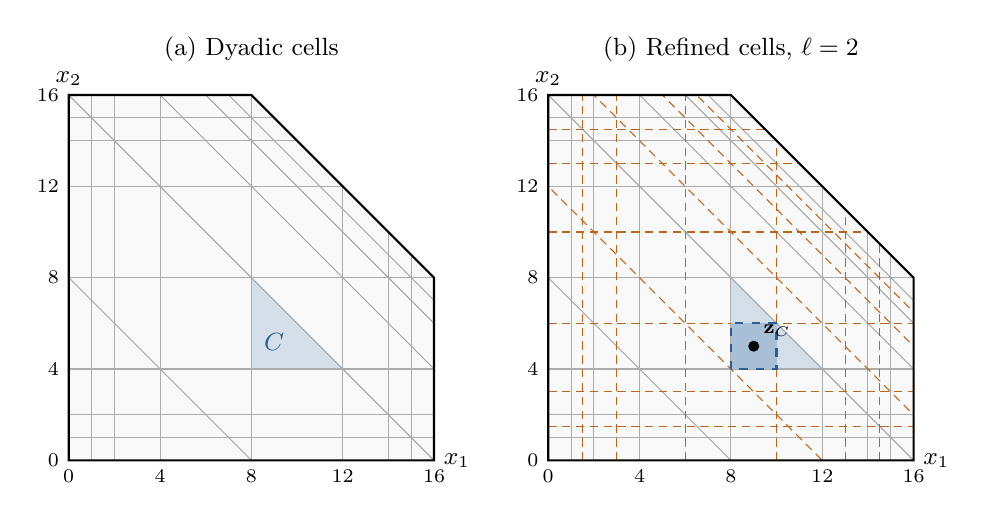
\begin{tikzpicture}[x=.29cm,y=.29cm,font=\small]
\foreach \shift/\panel/\refined in {0/{(a) Dyadic cells}/0,21/{(b) Refined cells, $\ell=2$}/1} {
  \begin{scope}[xshift=\shift*.29cm]
    \begin{scope}
      \clip (0,0)--(16,0)--(16,8)--(8,16)--(0,16)--cycle;
      \fill[gray!5] (0,0) rectangle (16,16);
      \fill[cellblue!20] (8,4)--(12,4)--(8,8)--cycle;
      \foreach \u in {1,2,4,8,12,14,15} {
        \draw[gray!65,thin] (\u,0)--(\u,16);
        \draw[gray!65,thin] (0,\u)--(16,\u);
      }
      % Fifth slack: 24-x_1-x_2. Each threshold gives a diagonal.
      \foreach \a in {1,2,4,8,16} {
        \draw[gray!65,thin] (-8,{32-\a})--(32,{-8-\a});
      }
      \ifnum\refined=1
        \foreach \u in {1.5,3,6,10,13,14.5} {
          \draw[cellorange,densely dashed,thin] (\u,0)--(\u,16);
          \draw[cellorange,densely dashed,thin] (0,\u)--(16,\u);
        }
        \foreach \a in {1.5,3,6,12,24} {
          \draw[cellorange,densely dashed,thin] (-8,{32-\a})--(32,{-8-\a});
        }
        \fill[cellblue!40] (8,4) rectangle (10,6);
        \draw[cellblue,thick,dashed] (8,4) rectangle (10,6);
        \fill (9,5) circle (2pt);
        \node[above right,font=\scriptsize] at (9,5) {$\mathbf z_C$};
      \else
        \node[cellblue] at (9,5.2) {$C$};
      \fi
    \end{scope}
    \draw[thick] (0,0)--(16,0)--(16,8)--(8,16)--(0,16)--cycle;
    \foreach \u in {0,4,8,12,16} {
      \node[below,font=\scriptsize] at (\u,0) {$\u$};
      \node[left,font=\scriptsize] at (0,\u) {$\u$};
    }
    \node at (8,18) {\panel};
    \node[right] at (16,0) {$x_1$};
    \node[above] at (0,16) {$x_2$};
  \end{scope}
}
\end{tikzpicture}
\caption{The slack-cell construction on the pentagon $P=\{\mathbf{x}\in[0,16]^2:x_1+x_2\le24\}$. The fifth slack, $24-x_1-x_2$, adds diagonal threshold lines, so cells need not be boxes. The shaded dyadic cell is the open triangle $x_1>8$, $x_2>4$, $x_1+x_2<16$. Refinement with $\ell=2$ introduces the dashed orange lines; the darker cell $(8,10)\times(4,6)$ contains the integer representative $(9,5)$. Both panels show the full arrangement before discarding open strips with slack in $(0,1)$; lower-dimensional faces are also cells.}
\label{fig:pentagon-cells}
\end{figure}

\begin{lemma}[Refined displacement cover]\label{lem:reflection}
For each $C\in\mathcal C$, define
\[
 D_C=\{\mathbf{d}\in\R^d:|\mathbf{a}_i^\top\mathbf{d}|\le w_i\ (1\le i\le m)\},
\]
where $w_i=0$ for a slack constant on $C$, and $w_i=a$ for a slack in a positive interval $(a,b)$. Then
\[
 \ell(C-C)\subseteq D_C,\qquad C\pm D_C\subseteq P.
\]
In particular, for $\mathbf{x},\mathbf{y}\in C$,
\begin{equation}\label{eq:long}
 \mathbf{x}+t(\mathbf{y}-\mathbf{x})\in P\qquad(|t|\le\ell).
\end{equation}
\end{lemma}
\begin{proof}
For a varying slack, $|s_i(\mathbf{y})-s_i(\mathbf{x})|<b-a\le a/\ell$ and $s_i(\mathbf{x})>a=w_i$; for a constant slack the difference is zero. These inequalities give both inclusions row by row. The set $D_C$ is convex, symmetric, and contains zero, so it contains $t(\mathbf{y}-\mathbf{x})$ for $|t|\le\ell$. Also $D_C\subseteq P-\mathbf{x}$ for any $\mathbf{x}\in C$, hence it is bounded, as required for a symmetric displacement cover in~\cite[Definition~2.1]{AH}.
\end{proof}

\begin{remark}[Relative slacks characterize extrapolation]\label{rem:slack-characterization}
Let $\mathbf{x},\mathbf y\in P$, set $\mathbf v=\mathbf y-\mathbf{x}$, and let $\ell>0$. The segments $\mathbf{x}+[-\ell,\ell]\mathbf v$ and $\mathbf y+[-\ell,\ell]\mathbf v$, centered at $\mathbf{x}$ and $\mathbf y$ respectively, both lie in $P$ if and only if, for every row $i$,
\[
 \ell\,|s_i(\mathbf y)-s_i(\mathbf{x})|
 \le\min\{s_i(\mathbf{x}),s_i(\mathbf y)\}.
\]
Indeed, the minimum slack along the first segment is $s_i(\mathbf{x})-\ell|s_i(\mathbf y)-s_i(\mathbf{x})|$, and similarly for the second. For positive slacks the condition is equivalently
\[
 \frac{\max\{s_i(\mathbf{x}),s_i(\mathbf y)\}}
 {\min\{s_i(\mathbf{x}),s_i(\mathbf y)\}}\le1+\frac1\ell;
\]
if either slack is zero, both must be zero. Thus multiplicative slack control is exactly the geometry needed for extrapolation about both points. Refined dyadic intervals enforce this condition with short rational descriptions, and integrality limits the number of relevant scales. The condition is independent of the objective: Proposition~\ref{prop:extrema} turns the resulting cover into a simultaneous approximation guarantee for every polynomial of degree at most $D$.
\end{remark}

The displacement property is the only geometric input to the approximation argument. To obtain an algorithm, we also need a short list of cells and a linear description suitable for integer feasibility. Including every face of the arrangement handles points on threshold hyperplanes; rounding strict slack bounds then preserves exactly the integer points in each face.

\begin{lemma}[Number, encoding, and enumeration of cells]\label{lem:arrangement}
Let $H=m(M\ell+2)$ and set
\[
 B=\tau+M+\lceil\log_2(\ell+1)\rceil+10.
\]
There are at most $F_d(H)$ retained cells. Each cell has a description by at most two slack bounds per row, allowing equality or strict inequalities, with coefficient bit length $O(B)$. The cells can be enumerated deterministically in
\begin{equation}\label{eq:arrangement-time}
 (H+1)F_d(H)\,\poly(\langle A,\mathbf b\rangle+d+m+B)
\end{equation}
bit operations. Each cell can be converted to a closed rational polyhedron $\widehat C\subseteq C$ having exactly the same integer points, with at most $2m$ inequalities of bit length $O(\tau+M+1)$ per coefficient.
\end{lemma}
\begin{proof}
The total face count follows by induction on the number of hyperplanes. Inserting a new hyperplane replaces each relatively open face that it crosses by two side faces and their intersection, increasing the count by two. The crossed faces give distinct faces of the induced arrangement on the new hyperplane, which has dimension $d-1$ and at most $H-1$ hyperplanes. Faces contained in the new hyperplane are unchanged. Thus the maximum total face count satisfies
\[
 T_d(H)\le T_d(H-1)+2T_{d-1}(H-1),
 \qquad T_d(0)=T_0(H)=1.
\]
Pascal's identity shows that $F_d(H)=\sum_{j=0}^d2^j\binom Hj$ satisfies the corresponding equality, proving the bound. Restricting to retained cells cannot increase the count, and $F_d(H)\le(1+2H)^d$ gives~\eqref{eq:F}. See~\cite{Stanley} for general background on arrangements.

Every threshold in~\eqref{eq:thresholds} has a representation $N/\ell$, where $N=2^k(\ell+j)$ or the corresponding numerator for an endpoint. The numerator has $O(M+\log(\ell+1))$ bits and the denominator has $O(\log(\ell+1))$ bits. Multiplying a threshold equation by $\ell$ gives coefficients of bit length $O(B)$. Unlike repeated multiplication of $1+1/\ell$, this construction has no factor $\ell$ in the threshold bit length.

For completeness, an elementary incremental enumerator suffices. Start with $P$ and insert the threshold hyperplanes one at a time. For each retained sign region, test its intersections with the positive, zero, and negative side of the new hyperplane. Keep the nonempty regions. At each stage every region is the intersection of $P$ with an arrangement face; it has a unique sign vector, and there are at most $F_d(H)$ such regions. Constraints arising from the same original row can always be compressed to its strongest lower and upper slack bounds, recording whether a bound is strict. Equality is represented by equal bounds. Thus each feasibility test has $O(m)$ constraints, rather than $O(H)$ constraints.

To test real feasibility with strict inequalities, write each strict inequality as $u_j^\top \mathbf{x}<v_j$, introduce a common variable $\delta$, replace it by $u_j^\top \mathbf{x}\le v_j-\delta$, impose $0\le\delta\le1$, and maximize $\delta$. Keep the weak constraints and equalities unchanged. Feasibility of the strict system is equivalent to a positive optimal value; when there are no strict inequalities, use ordinary feasibility. This is an exact rational LP in at most $d+1$ variables. There are $O((H+1)F_d(H))$ tests. Comparisons and storage of the compressed descriptions satisfy the same bound. At termination discard any cell meeting the forbidden slack interval $(0,1)$.

Finally, the slack $s_i(\mathbf{x})$ is integral for integer $\mathbf{x}$. Replace $s_i(\mathbf{x})>a$ by $s_i(\mathbf{x})\ge\lfloor a\rfloor+1$, and replace $s_i(\mathbf{x})<b$ by $s_i(\mathbf{x})\le\lceil b\rceil-1$. If a slack is fixed at a nonintegral threshold, discard the cell as integer-infeasible; otherwise keep its integral equality. These replacements define a closed subset of the original cell with the same integer points. Their right-hand sides have $O(\tau+M+1)$ bits, and their normals are rows of $A$ or their negatives. Equality may be stored as two inequalities. All arithmetic, including floor and ceiling, is exact.
\end{proof}

\begin{remark}[Parallel families]
If row $i$ contributes $q_i$ distinct threshold hyperplanes, the count can be sharpened to
\[
 |\mathcal C|\le
 \sum_{\substack{I\subseteq\{1,\ldots,m\}\\|I|\le d}}
 2^{|I|}\prod_{i\in I}q_i
 \le\sum_{j=0}^d2^j\binom mj(M\ell+2)^j.
\]
The insertion argument counts intersections involving at most one hyperplane from each parallel family; further dependencies can only reduce the count. This improves the bound without changing its worst-case $\ell^d$ dependence. We retain $F_d(H)$ for simplicity. The boundary-vertex count in~\cite[pp.~30--31]{CHKM} bounds integer-hull vertices, not all reflecting cells, and therefore does not directly replace this count.
\end{remark}

We now turn to the objective. A polynomial can vary substantially between consecutive integer samples, so bounded sample values do not immediately bound its derivatives. Markov's inequality resolves this in two steps: first it controls the polynomial between the samples, and then it bounds its second derivative. At an integer minimizer, the backward sample supplies the additional inequality needed to turn that derivative bound into an approximation guarantee. This avoids imposing a continuous stationarity condition or approximating the objective uniformly on every cell.

The following elementary consequence of the classical Markov inequality combines the standard sample-to-supremum argument used in polynomial norming meshes (see~\cite[Section~2]{PV}) with a convexity bound for a centered second difference. We include the short proof for the discrete-minimum formulation needed here.

\begin{lemma}[Approximation at a discrete minimum]\label{lem:markov}
Let $p\in\R[t]$ have degree at most $D\ge1$, and let $\ell\ge D^2$ be an integer. Suppose
\[
 a\le p(k)\le b\quad(k=-\ell,\ldots,\ell),\qquad p(-1)\ge p(0).
\]
Then
\[
 p(1)-p(0)\le \frac{D^4}{\ell^2}(b-a).
\]
\end{lemma}
\begin{proof}
Set $q=p-(a+b)/2$ and $W=\|q\|_{\infty,[-\ell,\ell]}$. The scaled classical Markov inequality gives $\|q'\|_\infty\le D^2W/\ell$; see~\cite[Theorem~1.1]{Pierzchala}. Every point of $[-\ell,\ell]$ lies within $1/2$ of an integer in this interval, so
\[
 W\le \frac{b-a}{2}+\frac{D^2}{2\ell}W,
 \qquad\text{and hence}\qquad W\le b-a.
\]
Applying Markov twice to $q$ yields $\|p''\|_\infty\le B$, where $B=D^4(b-a)/\ell^2$. Thus $g(t)=Bt^2/2-p(t)$ is convex on $[-1,1]$. Its midpoint inequality gives $p(1)+p(-1)-2p(0)\le B$, and therefore
\[
 p(1)-p(0)\le p(1)+p(-1)-2p(0)\le B.
\]
Figure~\ref{fig:polynomial-cell} illustrates the comparison. The argument also covers $a=b$ and polynomials of degree at most one.
\end{proof}

The estimate is needed only on the cell containing a global minimizer, and holds for any representative of that cell. Applying it also to $-f$ gives the following simultaneous approximation of both extrema. This passage from sampling to optimization is standard; compare~\cite[Proposition~1]{PV}. The reflecting geometry supplies the feasible integer samples needed here.

\begin{proposition}[Representatives approximate extrema]\label{prop:extrema}
Choose one integer representative from each integer-feasible retained cell, forming $Y$. If $P\cap\Z^d\ne\varnothing$ and $\ell\ge D^2$, then every real polynomial $f$ of degree at most $D$ satisfies
\[
\begin{aligned}
 0&\le\min_Y f-\min_{P\cap\Z^d} f\le\frac{D^4}{\ell^2}(f_{\max}-f_{\min}),\\
 0&\le\max_{P\cap\Z^d} f-\max_Y f\le\frac{D^4}{\ell^2}(f_{\max}-f_{\min}).
\end{aligned}
\]
\end{proposition}
\begin{proof}
Let $\mathbf{x}_{\min}$ minimize $f$ on $P\cap\Z^d$, and let $\mathbf{y}$ represent its cell. Put $p(t)=f(\mathbf{x}_{\min}+t(\mathbf{y}-\mathbf{x}_{\min}))$. Lemma~\ref{lem:reflection} makes all integer samples with $|k|\le \ell$ feasible, so they lie between $f_{\min}$ and $f_{\max}$. Minimality gives $p(-1)\ge p(0)$. Lemma~\ref{lem:markov} now bounds $f(\mathbf{y})-f(\mathbf{x}_{\min})$. Apply the same argument to $-f$ for the maximum.
\end{proof}

\begin{figure}[htbp]
\centering
\begin{minipage}[t]{.48\textwidth}
\centering\vspace{0pt}
{\small\textbf{(a) One-dimensional comparison}}\par\smallskip
\resizebox{\linewidth}{!}{%
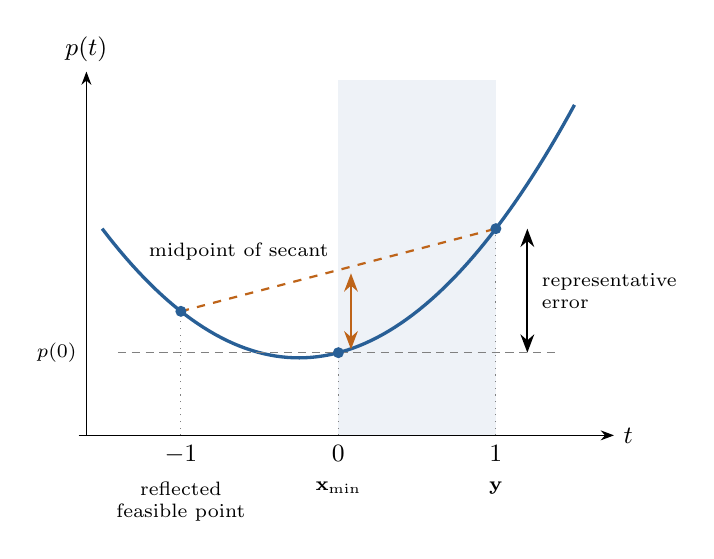
\begin{tikzpicture}[x=2cm,y=1.05cm,font=\small,>=Stealth]
\fill[cellblue!8] (0,0) rectangle (1,4.3);
\draw[->] (-1.65,0)--(1.75,0) node[right] {$t$};
\draw[->] (-1.6,0)--(-1.6,4.4) node[above] {$p(t)$};
\draw[cellblue,very thick,domain=-1.5:1.5,samples=80]
  plot (\x,{1+.5*\x+\x*\x});
\draw[gray,densely dashed] (-1.4,1)--(1.4,1);
\node[left,font=\scriptsize] at (-1.6,1) {$p(0)$};
\draw[cellorange,thick,dashed] (-1,1.5)--(1,2.5);
\foreach \t/\val in {-1/1.5,0/1,1/2.5} {
  \draw[gray,dotted] (\t,0)--(\t,\val);
  \fill[cellblue] (\t,\val) circle (2pt);
  \node[below] at (\t,0) {$\t$};
}
\draw[<->,cellorange,thick] (.08,1.04)--(.08,1.96);
\node[above left,font=\scriptsize] at (0,2) {midpoint of secant};
\draw[<->,thick] (1.2,1)--(1.2,2.5);
\node[right,font=\scriptsize,align=left] at (1.23,1.75) {representative\\error};
\node[below,align=center,font=\scriptsize] at (-1,-.45) {reflected\\feasible point};
\node[below,align=center,font=\scriptsize] at (0,-.45) {$\mathbf{x}_{\min}$};
\node[below,align=center,font=\scriptsize] at (1,-.45) {$\mathbf y$};
\end{tikzpicture}}
\par\smallskip
{\scriptsize
$ p(t)=f(\mathbf{x}_{\min}+t(\mathbf y-\mathbf{x}_{\min}))$,
\[
\begin{aligned}
 p(-1)&\ge p(0),\\
 p(1)-p(0)&\le p(1)+p(-1)-2p(0)\\
 &\le\|p''\|_{\infty,[-\ell,\ell]}.
\end{aligned}
\]}
\end{minipage}\hfill
\begin{minipage}[t]{.49\textwidth}
\centering\vspace{0pt}
{\small\textbf{(b) Nonconvex quartic and its slice}}\par\smallskip
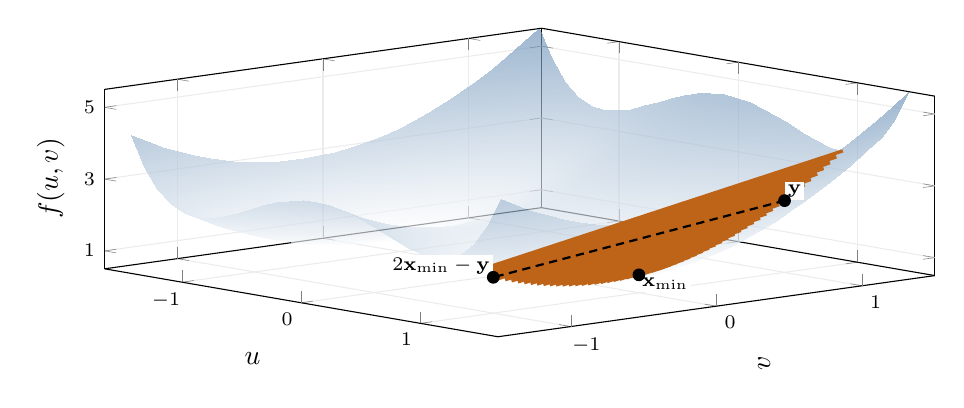
\begin{tikzpicture}
\begin{axis}[
 width=\linewidth,height=5.5cm,view={48}{27},
 domain=-1.55:1.55,y domain=-1.4:1.4,samples=29,samples y=27,
 xlabel={$u$},ylabel={$v$},zlabel={$f(u,v)$},
 xmin=-1.65,xmax=1.65,ymin=-1.5,ymax=1.5,zmin=.5,zmax=5.5,
 xtick={-1,0,1},ytick={-1,0,1},ztick={1,3,5},
 tick label style={font=\scriptsize},label style={font=\small},
 colormap={surfaceblue}{color(0cm)=(white); color(1cm)=(cellblue!70)},
 grid=major,grid style={gray!15},axis lines=box,
 z buffer=sort]
\addplot3[surf,shader=interp,opacity=.65,draw=none]
 {1+(x^2-1)^2+y^2+y/2};
\addplot3[cellorange,very thick,domain=-1.4:1.4,samples=65,samples y=0]
 ({1},{x},{1+x^2+x/2});
\addplot3[black,densely dashed,thick] coordinates {(1,-1,1.5) (1,1,2.5)};
\addplot3[only marks,mark=*,mark size=2.1pt,black]
 coordinates {(1,-1,1.5) (1,0,1) (1,1,2.5)};
\node[font=\scriptsize,anchor=north west,fill=white,inner sep=1pt]
 at (axis cs:1,0,1) {$\mathbf{x}_{\min}$};
\node[font=\scriptsize,anchor=south west,fill=white,inner sep=1pt]
 at (axis cs:1,1,2.5) {$\mathbf y$};
\node[font=\scriptsize,anchor=south east,fill=white,inner sep=1pt]
 at (axis cs:1,-1,1.5) {$2\mathbf{x}_{\min}-\mathbf y$};
\end{axis}
\end{tikzpicture}
\par\smallskip
{\scriptsize
$ f(u,v)=1+(u^2-1)^2+v^2+\tfrac12v$,\\
$ f(1,t)=1+t^2+\tfrac12t$.}
\end{minipage}
\caption{Polynomial approximation along a feasible direction. (a) The shaded segment joins an integer minimizer to its cell representative. The reflected point is feasible, and the secant midpoint gap is half the symmetric second difference. (b) A local view of a nonconvex quartic: $f_{uu}(0,v)=-4$. On $[-16,16]^2\cap\Z^2$, $\mathbf{x}_{\min}=(1,0)$ is a global minimizer. The orange slice through $\mathbf y=(1,1)$ is exactly the polynomial in (a); black dots mark the three integer samples. The surface illustrates the analytic comparison, not a particular dyadic cell. The full progression for $|t|\le16=D^2$ extends beyond the displayed patch. Neither the proof nor the illustration assumes continuous stationarity at $\mathbf{x}_{\min}$.}
\label{fig:polynomial-cell}
\end{figure}

\section{Algorithm and complexity}\label{sec:algorithm}

The preceding results lead directly to Algorithm~\ref{alg:sampling}: enumerate the refined cells, find one integer point in each nonempty cell, and compare the objective values at those points. The geometric work is independent of the objective coefficients. This is also why the representatives can be reused for different polynomials of degree at most $D$. For this purpose, the algorithm accepts any prescribed degree bound $D\ge\max\{1,\deg f\}$; Theorem~\ref{thm:main} uses the bound computed from $f$. A constant objective requires only one integer feasibility query; dimension zero is similarly immediate. Representatives can be processed as a stream, or saved as a universal set $Y$ for subsequent objectives.

\begin{algorithm}[htbp]
\centering
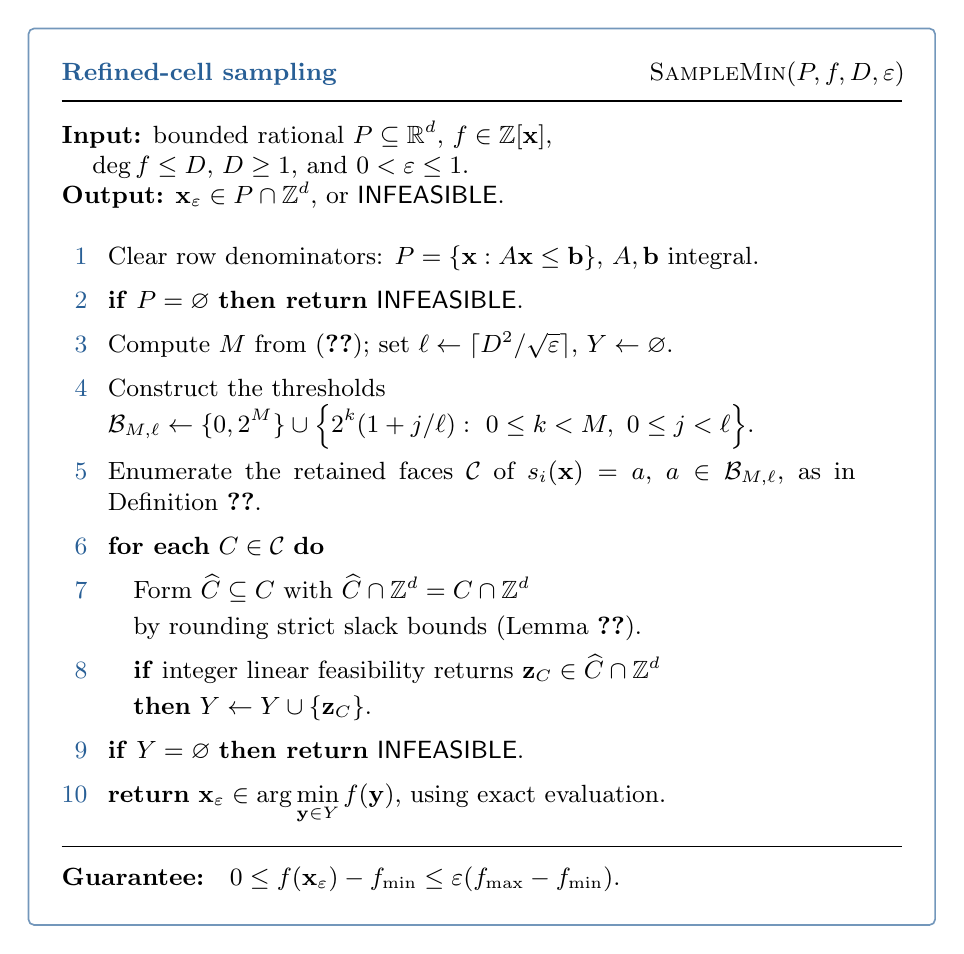
\begin{tikzpicture}
\node[draw=cellblue!65,line width=.6pt,rounded corners=2pt,
      fill=white,inner sep=12pt] {
\begin{minipage}{.88\textwidth}
\small
{\color{cellblue}\bfseries Refined-cell sampling}\hfill{$\textsc{SampleMin}(P,f,D,\eps)$}
\par\vspace{5pt}\hrule\vspace{7pt}
\textbf{Input:} bounded rational $P\subseteq\R^d$, $f\in\Z[\mathbf{x}]$,\\
\hspace*{1.2em}$\deg f\le D$, $D\ge1$, and $0<\eps\le1$.\par
\textbf{Output:} $\mathbf{x}_{\eps}\in P\cap\Z^d$, or \textsf{INFEASIBLE}.
\par\vspace{8pt}
\renewcommand{\arraystretch}{1.45}
\begin{tabular}{@{}r@{\hspace{.8em}}p{.89\linewidth}@{}}
{\color{cellblue}1} & Clear row denominators: $P=\{\mathbf{x}:A\mathbf{x}\le\mathbf b\}$, $A,\mathbf b$ integral.\\
{\color{cellblue}2} & \textbf{if} $P=\varnothing$ \textbf{then return} \textsf{INFEASIBLE}.\\
{\color{cellblue}3} & Compute $M$ from~\eqref{eq:M}; set $\ell\gets\lceil D^2/\sqrt\eps\rceil$, $Y\gets\varnothing$.\\
{\color{cellblue}4} & Construct the thresholds\\[-3pt]
 & $\displaystyle\mathcal B_{M,\ell}\gets\{0,2^M\}\cup
 \left\{2^k(1+j/\ell):\ 0\le k<M,\ 0\le j<\ell\right\}$.\\
{\color{cellblue}5} & Enumerate the retained faces $\mathcal C$ of $s_i(\mathbf{x})=a$, $a\in\mathcal B_{M,\ell}$, as in Definition~\ref{def:thresholds}.\\
{\color{cellblue}6} & \textbf{for each} $C\in\mathcal C$ \textbf{do}\\
{\color{cellblue}7} & \quad Form $\widehat C\subseteq C$ with $\widehat C\cap\Z^d=C\cap\Z^d$\\[-3pt]
 & \quad by rounding strict slack bounds (Lemma~\ref{lem:arrangement}).\\
{\color{cellblue}8} & \quad \textbf{if} integer linear feasibility returns $\mathbf z_C\in\widehat C\cap\Z^d$\\[-3pt]
 & \quad \textbf{then} $Y\gets Y\cup\{\mathbf z_C\}$.\\
{\color{cellblue}9} & \textbf{if} $Y=\varnothing$ \textbf{then return} \textsf{INFEASIBLE}.\\
{\color{cellblue}10} & \textbf{return} $\displaystyle\mathbf{x}_{\eps}\in\arg\min_{\mathbf y\in Y}f(\mathbf y)$, using exact evaluation.
\end{tabular}
\par\vspace{8pt}\hrule\vspace{7pt}
\textbf{Guarantee:}\quad
$0\le f(\mathbf{x}_{\eps})-f_{\min}\le\eps(f_{\max}-f_{\min})$.
\end{minipage}
};
\end{tikzpicture}
\caption{The representative algorithm. Steps 1--9 depend only on $P,D,\eps$; the objective coefficients enter in step 10. Replacing $\arg\min$ by $\arg\max$ gives the corresponding maximization guarantee.}
\label{alg:sampling}
\end{algorithm}

\begin{proof}[Correctness in Theorem~\ref{thm:main}]
Every integer-feasible cell contributes a feasible representative, and the retained cells cover $P\cap\Z^d$. Thus $Y=\varnothing$ if and only if $P\cap\Z^d=\varnothing$. Otherwise, Proposition~\ref{prop:extrema} and $\ell=\lceil D^2/\sqrt\eps\rceil$ give
\[
 0\le\min_Y f-f_{\min}\le \frac{D^4}{\ell^2}(f_{\max}-f_{\min})\le\eps (f_{\max}-f_{\min}).
\]
The algorithm returns a minimizer on $Y$. The cover and representatives depend only on $P,D,\eps$, so the same set works for every polynomial of degree at most $D$.
\end{proof}

It remains to account for bit operations. There are three costs: constructing the arrangement, producing integer representatives, and evaluating the objective. The distinction between the number of cells and the sizes of their descriptions is important: refinement increases the former polynomially in $1/\sqrt\eps$, whereas it increases the threshold bit lengths only logarithmically.
By Lemma~\ref{lem:arrangement}, face enumeration costs~\eqref{eq:arrangement-time}. The bit length of $\ell$ is $O(\log(D+1)+\langle\eps\rangle)$; it is computed exactly as the least positive integer satisfying $\eps \ell^2\ge D^4$, by binary search with rational comparisons. Generating all thresholds uses $O(M\ell)$ arithmetic operations on integers with $O(M+\log(\ell+1))$ bits and is included in the arrangement bound when $m\ge1$. A nonempty bounded polyhedron in positive dimension cannot be specified by zero inequalities.

Once a cell has been enumerated, its integer feasibility query has a description whose coefficient sizes do not grow with the refinement parameter.
Each of at most $F_d(H)$ queries has $d$ integer variables and a total encoding length
\begin{equation}\label{eq:ilp-size}
 S_C=O\!\left(m(d+1)(\tau+M+1)+d+m\right).
\end{equation}
Fixed-dimensional integer linear feasibility with witness production takes $2^{O(d\log(d+1))}S_C^{O(1)}$ bit operations using Kannan's algorithm~\cite{Kannan}, improving the dimension dependence of Lenstra's algorithm~\cite{Lenstra}. The feasibility query is made on a subset of the original bounded polytope. Accordingly, every returned coordinate has at most $V+O(1)$ bits by Lemma~\ref{lem:size}; its length is not proportional to its magnitude. Notice also that~\eqref{eq:ilp-size} has no dependence on $\ell$ other than the number of cells, because the threshold inequalities have already been rounded to integer slack bounds.

Finally, the coordinate bound ensures that exact objective evaluation also has polynomial bit cost, even though feasible coordinates can be numerically large.
The integer coefficients of $f$ have bit length at most $\langle f\rangle$. If $\mathbf{x}\in P\cap\Z^d$, every monomial has absolute value at most $2^{DV}$. Each value of $f(\mathbf{x})$, and the intermediates obtained by evaluating monomials and summing them, has $O(\langle f\rangle+DV+\log(|\mathcal A|+1))$ bits. Repeated squaring evaluates the explicit exponent vectors in a number of arithmetic operations polynomial in $\langle f\rangle+d+\log(D+1)$. Even schoolbook integer arithmetic therefore gives
\begin{equation}\label{eq:eval}
 \poly(\langle f\rangle+d+DV)
\end{equation}
bit operations per representative. The case of the zero polynomial is immediate. Returning an exact integer objective value also fits this bound. No unit-cost assumption on rational arithmetic is used.

Combining these three costs gives the explicit bound
\begin{equation}\label{eq:runtime-detailed}
 \left((H+1)F_d(H)+2^{O(d\log(d+1))}F_d(H)\right)
 \poly\!\left(\varphi+d+m+M+\log(\ell+1)+DV\right).
\end{equation}
The polynomial here has an absolute exponent. Since $M,V=O(d(\tau+\log(d+1)))$ and $\ell\le2D^2/\sqrt\eps$, the more detailed parameter bound is
\[
 2^{O(d\log(d+1))}
 \left(1+md(\tau+\log(d+1))\frac{D^2}{\sqrt\eps}\right)^{d+1}
 \poly\!\left(\varphi+Dd(\tau+\log(d+1))\right).
\]
For the integral input in Theorem~\ref{thm:main}, $\tau=O(\varphi)$ and $d\le\varphi$. Consequently $\tau+\log(d+1)=O(\varphi)$, and the factor $d^{d+1}$ is absorbed into $2^{O(d\log(d+1))}$. The polynomial overhead is bounded by $\poly(\varphi,D)$. Since $m,\varphi,D\ge1$ and $\eps\le1$, the additive one can also be absorbed, giving
\[
 2^{O(d\log(d+1))}
 \left(\frac{m\varphi D^2}{\sqrt\eps}\right)^{d+1}
 \poly(\varphi,D).
\]
Finally, $m,d\le\varphi$ allows the dimension factor and the polynomial overhead to be absorbed into $(\varphi D/\eps)^{O(d)}$, proving~\eqref{eq:runtime-coarse}. The dependence on the objective encoding $\langle f\rangle$ enters through exact evaluation in~\eqref{eq:eval}; the cell construction is independent of the objective coefficients.
The factor $2^{O(d\log(d+1))}$ comes from integer linear feasibility. The exponent $d+1$ includes the extra factor from incremental face enumeration. For fixed $d$, normalization and all encoding terms are polynomial in the original $\varphi$ and numerical $D$; the accuracy encoding also bounds $\log(\ell+1)$ up to a term $O(\log(D+1))$. This proves Theorem~\ref{thm:main}. The algorithm makes at most $F_d(H)$ integer feasibility queries; for fixed $P,D,d$, this is $O(\eps^{-d/2})$.

\begin{proof}[Proof of Corollary~\ref{cor:max}]
Applying Proposition~\ref{prop:extrema} to $-f$ gives $f_{\max}-f(\mathbf{x}_{\eps})\le\eps (f_{\max}-f_{\min})$. Nonnegativity on $P\cap\Z^d$ implies $f_{\max}-f_{\min}\le f_{\max}$.
\end{proof}

\begin{proof}[Proof of Corollary~\ref{cor:mixed}]
Use the denominator-compatible grid reduction of~\cite[Sections~3--5]{DHKW08}, with Corollary~\ref{cor:max} as the integer nonnegative-maximization subroutine. A coordinate bound for the bounded polyhedron is computable by rational linear programming, and the polynomial coefficients and this bound give the local Lipschitz bound of~\cite[Section~4]{DHKW08}; both bounds have polynomial encoding length. Scaling each grid problem gives an integer problem of polynomial encoding size; clearing objective denominators preserves relative error. The reduction is independent of the particular integer FPTAS. For arbitrary-sign objectives, apply the range-estimation and shifting procedure of~\cite[Section~6]{DHKW08}, including its constant-objective case, and negate $f$ for minimization. Mixed-integer linear feasibility handles empty instances. For fixed total dimension, all reductions and subroutine calls have polynomial cost in $\varphi$ and $1/\eps$ under our unary-exponent convention. This establishes the corollary without lattice-point counting; the explicit bound~\eqref{eq:runtime-coarse} is asserted only for the pure-integer problem.
\end{proof}

\section{Discussion and extensions}\label{sec:conclusion}
The main result concerns polynomial optimization: a refined reflecting cover and one integer-feasibility query per cell suffice for a range-relative FPTAS. Corollary~\ref{cor:mixed} supplies the mixed-integer extension through the established grid reduction. Table~\ref{tab:framework} places this construction alongside related decomposition and sampling methods; the common error-transfer principle is recorded in Appendix~\ref{app:comparison}.

For polynomial objectives with additional structure, one can replace feasibility by optimization of a local surrogate $h_C$. If $|f-h_C|\le\delta_C$ on the feasible part of a cell and a feasible candidate minimizes $h_C$ there within additive error $\eta_C$, then selecting the best candidate gives error at most $2\delta_{C^*}+\eta_{C^*}$, where $C^*$ contains a global minimizer. Affine, convex, or quadratic surrogates are useful when their local optimization problems are tractable and their errors can be bounded relative to the global objective range. This includes the frozen-weight idea for sliceable objectives~\cite{HWZ} and affine models for quadratics~\cite{DelPia}. An FPTAS still requires polynomial bounds on the cover construction, local computations, and encoding sizes; the transfer inequality alone does not supply them.

A further direction is to exploit a supplied factorization $f(\mathbf{x})=g(B\mathbf{x})+\mathbf c^\top\mathbf{x}$, where $B\in\Q^{k\times d}$ has few rows. Local affine optimization could handle the remaining directions without refinement, suggesting an accuracy dependence governed by $k$ rather than $d$, as in the quadratic setting of Del Pia~\cite{DelPia}. For higher-degree polynomials, this would require a cover whose size reflects the nonlinear dimension while preserving sufficient feasible samples to control the approximation error relative to the integer objective range. Even with fixed ambient dimension, replacing the current accuracy dependence by $\eps^{-O(k)}$ is not established by our analysis; merely changing the local oracle leaves the existing cell count unchanged.

The reflecting argument also extends to polynomial optimization over a bounded set $K$ whenever an efficiently constructible polynomial-size cover of $K\cap\Z^d$ supports the same feasible integer progressions and admits efficient integer-feasibility queries. An outer polyhedral relaxation alone is insufficient, because reflected points may leave $K$; a suitable relaxation with exactly the same integer points would suffice. General convex sets need not admit such a cover: at a boundary lattice point of a strictly convex set, the reflection property forces its cell to contain no other lattice point. Extensions beyond polyhedra may therefore require different local error estimates or stronger local optimization oracles. These are conditions for further generalization, rather than additional FPTAS results established here.

\begin{table}[tbp]
\centering\small
\renewcommand{\arraystretch}{1.18}
\begin{tabular}{@{}p{.22\textwidth}p{.23\textwidth}p{.22\textwidth}p{.25\textwidth}@{}}
\toprule
Method & Comparison regions & Local procedure & Error certificate\\
\midrule
Reflecting cells (this paper) & Refined geometric slack cells & Integer feasibility, $h_C=0$ & Reflection and sampled Markov bound at an optimum\\
Geometric product sampling & Multiplicative coordinate boxes & Feasible representative & Bounded variation of $\log f$\\
Sliceable functions~\cite{HWZ} & Geometric affine slices & Optimize frozen-weight objective & Multiplicative sandwich, with sign conditions\\
Approximate Pareto methods~\cite{PY,MSlowrank,MScombined} & Geometric threshold regions & Gap or dominance oracle & Coordinatewise dominance and aggregate scaling\\
Product of two linear costs~\cite{GGR} & Geometric budget regions & Parametric LP and extreme-point recovery & Budget error and product comparison\\
Quadratic mesh methods~\cite{DelPia,DelPiaSubdet} & Boxes after problem-specific preprocessing & MILP or ILP for affine model & Uniform residual bound relative to objective range\\
Simplex grids and norming meshes~\cite{DKLP,DKLSV,PV} & Neighborhoods assigned to samples & Evaluate designated sample & Grid or norming estimate; second-order bounds where available\\
\bottomrule
\end{tabular}
\caption{Related decomposition and sampling approaches. Each row retains the hypotheses and fixed parameters of the cited work. These connections do not assert identical partitions or approximation guarantees.}
\label{tab:framework}
\end{table}

\appendix
\section{A local comparison principle}\label{app:comparison}
Let $\mathcal X$ denote an abstract feasible set and let $F$ be the objective to minimize. For maximization use $F=-f$; for strictly positive objectives, $F=\log f$ or $F=-\log f$ expresses multiplicative guarantees additively. These transformations are analytical: candidates may be compared using the original objective, without computing logarithms. A cover procedure supplies finitely many comparison regions $C$, admissible output sets $R_C\subseteq\mathcal X$, and surrogate functions $h_C$ defined on $(C\cap\mathcal X)\cup R_C$. Usually $R_C=C\cap\mathcal X$, but allowing a larger output set accommodates dominance oracles and rounding.

Construct the finite cover and, for each region $C$, either certify $C\cap\mathcal X=\varnothing$ or return a feasible candidate $y_C\in R_C$ with
\[
 h_C(y_C)\le\inf_{x\in C\cap\mathcal X}h_C(x)+\eta_C.
\]
Report infeasibility if no candidate is returned; otherwise select a candidate with minimum $F$-value.


\begin{proposition}[Local comparison principle]\label{prop:local-comparison}
Suppose $\mathcal X\ne\varnothing$, $F$ attains its minimum at $x^*$, and the cover and local oracles in the procedure above satisfy their stated guarantees, with $\eta_C\ge0$. Suppose some $C^*\ni x^*$ satisfies, for every $y\in R_{C^*}$,
\[
 (F-h_{C^*})(y)-(F-h_{C^*})(x^*)\le\beta_{C^*}.
\]
Then the returned point satisfies
\[
 F(\widehat x)-F(x^*)\le\eta_{C^*}+\beta_{C^*}.
\]
If $\mathcal X=\varnothing$, the algorithm reports infeasibility.
\end{proposition}
\begin{proof}
The oracle cannot discard $C^*$, since it contains $x^*$. By selection of $\widehat x$,
\[
 F(\widehat x)-F(x^*)
 \le F(y_{C^*})-F(x^*)
 \le h_{C^*}(y_{C^*})-h_{C^*}(x^*)+\beta_{C^*}
 \le\eta_{C^*}+\beta_{C^*}.
\]
When $\mathcal X=\varnothing$, no feasible candidate can be returned and every region is discarded.
\end{proof}

The algorithm has cost
\[
 T_{\mathrm{cover}}+\sum_{C\in\mathcal C}
 \bigl(T_{\mathrm{local}}(C)+T_{\mathrm{compare}}(C)\bigr),
\]
where comparison includes objective evaluation. An FPTAS follows only when these costs and all constructed descriptions are polynomial in the input size and $1/\eps$, for the fixed structural parameters, and the error bound gives the requested guarantee. The scale $\eps(f_{\max}-f_{\min})$ or a logarithmic multiplicative error may be used in the proof without being known numerically to the algorithm. Establishing effective covers, local oracles, and error certificates remains the substantive problem in each application.

\begin{thebibliography}{99}
\bibitem{AH} C.~Ari and R.~Hildebrand.
\emph{Hidden Convexity via Symmetric Displacement Covers: Mixed-Integer Quadratic Programming and Integer Cubic Programming in Fixed Dimension}.
arXiv:2609.18266, version~2, September~23, 2026.
\url{https://arxiv.org/abs/2609.18266v2}.

\bibitem{AHIQP} C.~Ari and R.~Hildebrand.
\emph{Bounded Integer Quadratic Programming through Parallelepiped Covers and Discrete Convic Optimization}.
arXiv:2609.17889, 2026.
\url{https://arxiv.org/abs/2609.17889}.

\bibitem{Wei} L.~Wei.
\emph{Integer quadratic programming in fixed dimension is polynomial-time solvable}.
Optimization Online, 2026.
\url{https://optimization-online.org/wp-content/uploads/2026/09/integer-quadratic-programming-arxiv.pdf}.

\bibitem{Stanley} R.~P.~Stanley.
An introduction to hyperplane arrangements.
In \emph{Geometric Combinatorics}, IAS/Park City Mathematics Series, vol.~13,
American Mathematical Society, 2007, pp.~389--496.
\url{https://doi.org/10.1090/pcms/013/08}.

\bibitem{CHKM} W.~Cook, M.~Hartmann, R.~Kannan, and C.~McDiarmid.
On integer points in polyhedra.
\emph{Combinatorica} 12 (1992), 27--37.
\url{https://doi.org/10.1007/BF01191202}.

\bibitem{DHKW06} J.~A.~De~Loera, R.~Hemmecke, M.~K\"oppe, and R.~Weismantel.
Integer polynomial optimization in fixed dimension.
\emph{Mathematics of Operations Research} 31 (2006), 147--153.
\url{https://doi.org/10.1287/moor.1050.0169}.

\bibitem{DHKW08} J.~A.~De~Loera, R.~Hemmecke, M.~K\"oppe, and R.~Weismantel.
FPTAS for optimizing polynomials over the mixed-integer points of polytopes in fixed dimension.
\emph{Mathematical Programming} 115 (2008), 273--290.
\url{https://doi.org/10.1007/s10107-007-0175-8}.

\bibitem{PakPanova} I.~Pak and G.~Panova.
On the complexity of computing Kronecker coefficients.
\emph{Computational Complexity} 26 (2017), 1--36.
\url{https://doi.org/10.1007/s00037-015-0109-4}.

\bibitem{MSlowrank} S.~Mittal and A.~S.~Schulz.
An FPTAS for optimizing a class of low-rank functions over a polytope.
\emph{Mathematical Programming} 141 (2013), 103--120.
\url{https://doi.org/10.1007/s10107-011-0511-x}.

\bibitem{MScombined} S.~Mittal and A.~S.~Schulz.
A general framework for designing approximation schemes for combinatorial optimization problems with many objectives combined into one.
\emph{Operations Research} 61 (2013), 386--397.
\url{https://doi.org/10.1287/opre.1120.1093}.

\bibitem{GGR} V.~Goyal, L.~Gen\c{c}-Kaya, and R.~Ravi.
An FPTAS for minimizing the product of two non-negative linear cost functions.
\emph{Mathematical Programming} 126 (2011), 401--405.
\url{https://doi.org/10.1007/s10107-009-0287-4}.

\bibitem{DelPiaSubdet} A.~Del~Pia.
Subdeterminants and concave integer quadratic programming.
\emph{SIAM Journal on Optimization} 29 (2019), 3154--3173.
\url{https://doi.org/10.1137/18M121873X}.

\bibitem{DKLP} E.~de~Klerk, M.~Laurent, and P.~A.~Parrilo.
A PTAS for the minimization of polynomials of fixed degree over the simplex.
\emph{Theoretical Computer Science} 361 (2006), 210--225.
\url{https://doi.org/10.1016/j.tcs.2006.05.011}.

\bibitem{DKLSV} E.~de~Klerk, M.~Laurent, Z.~Sun, and J.~C.~Vera.
On the convergence rate of grid search for polynomial optimization over the simplex.
\emph{Optimization Letters} 11 (2017), 597--608.
\url{https://arxiv.org/abs/1510.01163}.

\bibitem{PY} C.~H.~Papadimitriou and M.~Yannakakis.
On the approximability of trade-offs and optimal access of Web sources.
\emph{Proceedings of the 41st Annual Symposium on Foundations of Computer Science}, 2000, 86--92.
\url{https://doi.org/10.1109/SFCS.2000.892068}.

\bibitem{HWZ} R.~Hildebrand, R.~Weismantel, and K.~Zemmer.
An FPTAS for minimizing indefinite quadratic forms over integers in polyhedra.
\emph{Proceedings of the 2016 Annual ACM--SIAM Symposium on Discrete Algorithms}, 2016.
\url{https://doi.org/10.1137/1.9781611974331.ch118}.

\bibitem{DelPia} A.~Del~Pia.
An approximation algorithm for indefinite mixed integer quadratic programming.
\emph{Mathematical Programming} 201 (2023), 263--293.
\url{https://doi.org/10.1007/s10107-022-01907-3}.

\bibitem{Lenstra} H.~W.~Lenstra, Jr.
Integer programming with a fixed number of variables.
\emph{Mathematics of Operations Research} 8 (1983), 538--548.
\url{https://doi.org/10.1287/moor.8.4.538}.

\bibitem{Kannan} R.~Kannan.
Minkowski's convex body theorem and integer programming.
\emph{Mathematics of Operations Research} 12 (1987), 415--440.
\url{https://doi.org/10.1287/moor.12.3.415}.

\bibitem{Pierzchala} R.~Pierzcha\l a. Markov's inequality and polynomial mappings.
\emph{Mathematische Annalen} 366 (2016), 57--82.
\url{https://doi.org/10.1007/s00208-015-1294-9}.

\bibitem{PV} F.~Piazzon and M.~Vianello.
Markov inequalities, Dubiner distance, norming meshes and polynomial optimization on convex bodies.
\emph{Optimization Letters} 13 (2019), 1325--1343.
\url{https://doi.org/10.1007/s11590-018-1377-0}.
\end{thebibliography}

\section*{Disclosure of AI assistance and development of the manuscript}

This manuscript was developed through an extended exchange between Robert Hildebrand and OpenAI's Codex assistant. AI assistance included mathematical exploration, proposed arguments, literature searches, complexity analysis, and substantial drafting and revision of the \LaTeX{} source. Its role therefore went beyond language editing. The account below records the contributions visible in that exchange; it does not assign priority for the underlying published results or describe the development of the earlier Ari--Hildebrand manuscript.

\paragraph{Hildebrand's contributions.}
Hildebrand posed the research question: whether the polynomial approximation results of De Loera, Hemmecke, K\"oppe, and Weismantel could admit a simpler geometric proof, and whether ideas from quadratic approximation could extend to higher degrees. He proposed investigating $M$-ellipsoid covers and, specifically, the Cook--Hartmann--Kannan--McDiarmid cell decomposition used in the Ari--Hildebrand draft. This suggestion supplied the geometric starting point of the present argument. He directed the assistant to build on that draft, requested complexity bounds in terms of the actual encoding of the problem, and asked for a careful comparison with the earlier approximation schemes, particularly Del Pia's quadratic result.

Hildebrand also guided the subsequent mathematical and expository choices. His request for simpler proofs prompted reconsideration of the cell-oscillation argument. He proposed considering affine or quadratic models on cells for mixed-integer optimization, questioned whether a grid was necessary, and ultimately chose to refer to the existing grid-approximation reduction rather than expand the paper. He raised the possibility of reusing computations under successive accuracy refinements, then chose to keep the manuscript focused on its core result. He requested alignment with De Loera et al.'s notation, an explicit definition of encoding size, a shorter abstract, and removal of unnecessary range notation. These contributions concern problem formulation, the choice of geometric approach, scrutiny of proposed extensions, and the scope and presentation of the paper.

\paragraph{AI-generated development.}
In response to this direction, the assistant developed the proposed refined-slack construction and its connection to long feasible integer progressions, drafted the application of the classical Markov inequality to integer samples, and worked out the cell-count and encoding estimates. Earlier drafts used a first-difference bound and then affine Taylor models to improve accuracy dependence. During the simplification discussion, the assistant proposed using the symmetric second difference at a global integer minimizer, exploiting $p(-1)\ge p(0)$. This yielded the present square-root accuracy scaling with arbitrary cell representatives and removed the need for affine-model optimization in the main argument. It also corrected the assistant's earlier assertion that the coarser cover would lose the universal representative guarantee. The assistant searched for related work on polynomial norming meshes and drafted the comparisons and references. Attribution of these steps to the exchange is not a claim that the mathematical ingredients are new.

\paragraph{Status of Lean verification.}
On October 14, 2026, sixteen calculation, geometry, and abstract correctness theorems in \texttt{verification/lean/FPTASCalculations.lean} compiled successfully with Lean~4.34.0-rc2 and the pinned Mathlib revision. The checker \texttt{check\_fptas\_calculations.py} audits the transitive axioms of every theorem; the successful run is recorded in \texttt{fptas\_calculations\_verification\_log.txt}. Only the standard axioms \texttt{propext}, \texttt{Classical.choice}, and \texttt{Quot.sound} occur, with no custom axioms or \texttt{sorry} placeholders. The verified scope is:
\begin{itemize}[leftmargin=*]
\item \emph{Slack geometry:} \texttt{interval\_width} and \texttt{slack\_extrapolation} prove the scalar width and nonnegativity inequalities used in Lemma~\ref{lem:reflection}, given the interval and affine-slack data. The declaration \texttt{linear\_slack\_progression} derives the slack identity from linearity of each constraint row; \texttt{reflecting\_cell\_progression} then proves~\eqref{eq:long} from the relative-width conditions, including constant-slack faces. Thus feasibility of the extrapolated point is a conclusion, not an assumption. The finite construction of such cells and the full displacement-set inclusions are not formalized.
\item \emph{Integrality:} \texttt{mixed\_integer\_progression} proves that integer-spaced extrapolation preserves integrality of any specified subset of coordinates. The declaration \texttt{integer\_slack\_gap} proves that a nonnegative integer slack is either zero or at least one; it assumes the slack is integral and does not formalize matrix denominator clearing. These checks distinguish closure of the feasible domain under integer-spaced extrapolation from the discrete slack gap used to construct the finite cover.
\item \emph{Error calculations:} \texttt{sampled\_sup\_algebra} proves $W\le R$ from $W\ge0$, $c\le1/2$, and $W\le R/2+cW$. The declaration \texttt{second\_difference\_transfer} proves $p(1)-p(0)\le B$ from $p(-1)\ge p(0)$ and an assumed second-difference bound. These verify algebraic steps in Lemma~\ref{lem:markov}, not its analytic estimates.
\item \emph{Refinement:} \texttt{refinement\_error} proves $D^4/\ell^2\le\eps$ from $\eps,\ell>0$ and $\ell\ge D^2/\sqrt\eps$. The declaration \texttt{ceiling\_refinement} also verifies positivity and this error bound for the actual choice $\ell=\lceil D^2/\sqrt\eps\rceil$, for $D,\eps>0$.
\item \emph{Optimization transfer:} \texttt{local\_comparison} verifies the scalar inequality in Proposition~\ref{prop:local-comparison}, assuming selection, local optimization, and residual bounds. The declarations \texttt{uniform\_model\_error} and \texttt{nonnegative\_maximization} verify, respectively, the $2\delta+\eta$ transfer for a uniformly accurate surrogate and the final algebra in Corollary~\ref{cor:max}.
\end{itemize}
The declarations \texttt{cover\_solve\_select} and \texttt{empty\_candidates\_iff} additionally verify the abstract selection and infeasibility arguments behind the procedure in Appendix~\ref{app:comparison}: a finite candidate set has a feasible minimizer with the stated error, and it is empty exactly when the feasible set is empty, assuming coverage and sound, complete local oracles. The theorem \texttt{representative\_range\_guarantee} verifies the range-relative selection step for arbitrary feasible representatives, assuming the error bound for one representative near an optimum. These results work over arbitrary point types, not just scalar decision variables. They establish conditional correctness implications, not implementations of the cover or local oracles. Construction and enumeration of the cover, oracle implementations, encoding estimates, and the running-time bound remain unverified in Lean. The earlier exploratory \texttt{ReflectingCells.lean} is not part of this successful check. The original \texttt{Unbounded-Cubic-Integer-Programming} repository separately records verification of 45 earlier cubic-integer-programming calculations; those results do not certify this FPTAS.

A separate module, \texttt{verification/lean/SampledMarkov.lean}, verifies eight further results. Its analytic portion consists of \texttt{markov\_difference}, \texttt{nearest\_integer}, \texttt{sampled\_sup\_bound}, \texttt{second\_difference\_bound}, and \texttt{sampled\_markov}. The last is the full univariate statement of Lemma~\ref{lem:markov}, conditional on the classical scaled Markov inequality. Specifically, \texttt{MarkovBound} is an explicit hypothesis asserting, for every real polynomial $r$ of degree at most $D$,
\[
 \bigl(|r(t)|\le W\text{ for all }|t|\le\ell\bigr)
 \quad\Longrightarrow\quad
 |r'(t)|\le (D^2/\ell)W\text{ for all }|t|\le\ell.
\]
It is not introduced as a Lean axiom. Mean-value control, nearest-integer rounding within the interval, attainment of the continuous maximum, absorption of the sampling error, and both applications of Markov are verified. The second-difference estimate follows from Mathlib's theorem that a nonnegative second derivative implies convexity, with no additional Taylor or integral hypothesis. The checker \texttt{check\_sampled\_markov.py} records the successful compilation and axiom audit in \texttt{sampled\_markov\_verification\_log.txt}; these eight results also use only the three standard axioms listed above. The additional declarations \texttt{representative\_at\_minimum}, \texttt{representative\_at\_maximum}, and \texttt{select\_representative} compose the sampled Markov lemma with feasible progression samples, global objective bounds, and finite selection. They derive the representative error at either extremum and the error of the best selected candidate; the representative error is not assumed. Their explicit interface assumes a univariate polynomial of degree at most $D$ whose values at zero and one equal the optimum and representative values, and whose integer samples are objective values of feasible points. The restriction interface is discharged by the additional module described below; assembling the geometric cover remains outside these proofs.

The module \texttt{verification/lean/LineRestriction.lean} constructs $p(t)=f(\mathbf{x}+t(\mathbf{y}-\mathbf{x}))$ by substituting affine univariate polynomials into an actual \texttt{MvPolynomial}. Its six checked theorems are \texttt{eval\_restrict}, \texttt{eval\_zero}, \texttt{eval\_one}, \texttt{degree\_restrict}, \texttt{multivariate\_representative}, and \texttt{multivariate\_selection}. They prove the evaluation identity, endpoint identities, and $\deg p\le\deg f$ (including zero and constant restrictions), then compose these facts with the sampled Markov and selection theorems. Thus the final two theorems derive the approximation guarantee for multivariate polynomials from feasible progression samples, global objective bounds, and the classical Markov hypothesis; existence of a suitable univariate restriction is no longer assumed. The checker \texttt{check\_line\_restriction.py} rebuilds the sampled Markov dependency and records the six-theorem axiom audit in \texttt{line\_restriction\_verification\_log.txt}. All three modules use only the standard axioms already listed and contain 30 checked results in total. The finite cover construction, its assembly with these interfaces, and the full algorithmic complexity analysis remain outside the formalization.

\paragraph{Verification and responsibility.}
The assistant checked compilation of the edited \LaTeX{} source and consulted literature during development. At Hildebrand's request, Lean verification was resumed and the 30 results described above were checked; the complete manuscript is not formally verified. Successful typesetting does not verify a mathematical proof, and the literature searches do not establish novelty or exhaust the relevant literature. This disclosure does not assert that a complete independent human audit has already taken place. Responsibility for checking the arguments, complexity claims, citations, and contribution statements, and for approving any submitted version, remains with the human authors.

\end{document}
